\documentclass[1p]{elsarticle_modified}
%\bibliographystyle{elsarticle-num}

%\usepackage[colorlinks]{hyperref}
%\usepackage{abbrmath_seonhwa} %\Abb, \Ascr, \Acal ,\Abf, \Afrak
\usepackage{amsfonts}
\usepackage{amssymb}
\usepackage{amsmath}
\usepackage{amsthm}
\usepackage{scalefnt}
\usepackage{amsbsy}
\usepackage{kotex}
\usepackage{caption}
\usepackage{subfig}
\usepackage{color}
\usepackage{graphicx}
\usepackage{xcolor} %% white, black, red, green, blue, cyan, magenta, yellow
\usepackage{float}
\usepackage{setspace}
\usepackage{hyperref}

\usepackage{tikz}
\usetikzlibrary{arrows}

\usepackage{multirow}
\usepackage{array} % fixed length table
\usepackage{hhline}

%%%%%%%%%%%%%%%%%%%%%
\makeatletter
\renewcommand*\env@matrix[1][\arraystretch]{%
	\edef\arraystretch{#1}%
	\hskip -\arraycolsep
	\let\@ifnextchar\new@ifnextchar
	\array{*\c@MaxMatrixCols c}}
\makeatother %https://tex.stackexchange.com/questions/14071/how-can-i-increase-the-line-spacing-in-a-matrix
%%%%%%%%%%%%%%%

\usepackage[normalem]{ulem}

\newcommand{\msout}[1]{\ifmmode\text{\sout{\ensuremath{#1}}}\else\sout{#1}\fi}
%SOURCE: \msout is \stkout macro in https://tex.stackexchange.com/questions/20609/strikeout-in-math-mode

\newcommand{\cancel}[1]{
	\ifmmode
	{\color{red}\msout{#1}}
	\else
	{\color{red}\sout{#1}}
	\fi
}

\newcommand{\add}[1]{
	{\color{blue}\uwave{#1}}
}

\newcommand{\replace}[2]{
	\ifmmode
	{\color{red}\msout{#1}}{\color{blue}\uwave{#2}}
	\else
	{\color{red}\sout{#1}}{\color{blue}\uwave{#2}}
	\fi
}

\newcommand{\Sol}{\mathcal{S}} %segment
\newcommand{\D}{D} %diagram
\newcommand{\A}{\mathcal{A}} %arc


%%%%%%%%%%%%%%%%%%%%%%%%%%%%%5 test

\def\sl{\operatorname{\textup{SL}}(2,\Cbb)}
\def\psl{\operatorname{\textup{PSL}}(2,\Cbb)}
\def\quan{\mkern 1mu \triangleright \mkern 1mu}

\theoremstyle{definition}
\newtheorem{thm}{Theorem}[section]
\newtheorem{prop}[thm]{Proposition}
\newtheorem{lem}[thm]{Lemma}
\newtheorem{ques}[thm]{Question}
\newtheorem{cor}[thm]{Corollary}
\newtheorem{defn}[thm]{Definition}
\newtheorem{exam}[thm]{Example}
\newtheorem{rmk}[thm]{Remark}
\newtheorem{alg}[thm]{Algorithm}

\newcommand{\I}{\sqrt{-1}}
\begin{document}

%\begin{frontmatter}
%
%\title{Boundary parabolic representations of knots up to 8 crossings}
%
%%% Group authors per affiliation:
%\author{Yunhi Cho} 
%\address{Department of Mathematics, University of Seoul, Seoul, Korea}
%\ead{yhcho@uos.ac.kr}
%
%
%\author{Seonhwa Kim} %\fnref{s_kim}}
%\address{Center for Geometry and Physics, Institute for Basic Science, Pohang, 37673, Korea}
%\ead{ryeona17@ibs.re.kr}
%
%\author{Hyuk Kim}
%\address{Department of Mathematical Sciences, Seoul National University, Seoul 08826, Korea}
%\ead{hyukkim@snu.ac.kr}
%
%\author{Seokbeom Yoon}
%\address{Department of Mathematical Sciences, Seoul National University, Seoul, 08826,  Korea}
%\ead{sbyoon15@snu.ac.kr}
%
%\begin{abstract}
%We find all boundary parabolic representation of knots up to 8 crossings.
%
%\end{abstract}
%\begin{keyword}
%    \MSC[2010] 57M25 
%\end{keyword}
%
%\end{frontmatter}

%\linenumbers
%\tableofcontents
%
\newcommand\colored[1]{\textcolor{white}{\rule[-0.35ex]{0.8em}{1.4ex}}\kern-0.8em\color{red} #1}%
%\newcommand\colored[1]{\textcolor{white}{ #1}\kern-2.17ex	\textcolor{white}{ #1}\kern-1.81ex	\textcolor{white}{ #1}\kern-2.15ex\color{red}#1	}

{\Large $\underline{12a_{1051}~(K12a_{1051})}$}

\setlength{\tabcolsep}{10pt}
\renewcommand{\arraystretch}{1.6}
\vspace{1cm}\begin{tabular}{m{100pt}>{\centering\arraybackslash}m{274pt}}
\multirow{5}{120pt}{
	\centering
	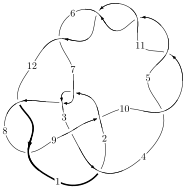
\includegraphics[width=112pt]{../../../GIT/diagram.site/Diagrams/png/1852_12a_1051.png}\\
\ \ \ A knot diagram\footnotemark}&
\allowdisplaybreaks
\textbf{Linearized knot diagam} \\
\cline{2-2}
 &
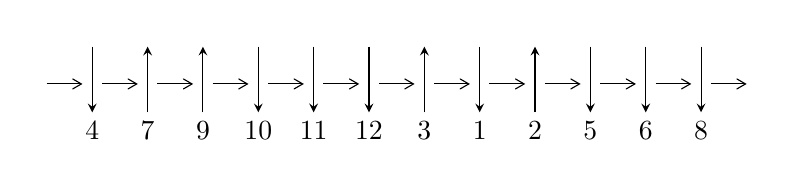
\begin{tikzpicture}[x=20pt, y=17pt]
	% nodes
	\node (C0) at (0, 0) {};
	\node (C1) at (1, 0) {};
	\node (C1U) at (1, +1) {};
	\node (C1D) at (1, -1) {4};

	\node (C2) at (2, 0) {};
	\node (C2U) at (2, +1) {};
	\node (C2D) at (2, -1) {7};

	\node (C3) at (3, 0) {};
	\node (C3U) at (3, +1) {};
	\node (C3D) at (3, -1) {9};

	\node (C4) at (4, 0) {};
	\node (C4U) at (4, +1) {};
	\node (C4D) at (4, -1) {10};

	\node (C5) at (5, 0) {};
	\node (C5U) at (5, +1) {};
	\node (C5D) at (5, -1) {11};

	\node (C6) at (6, 0) {};
	\node (C6U) at (6, +1) {};
	\node (C6D) at (6, -1) {12};

	\node (C7) at (7, 0) {};
	\node (C7U) at (7, +1) {};
	\node (C7D) at (7, -1) {3};

	\node (C8) at (8, 0) {};
	\node (C8U) at (8, +1) {};
	\node (C8D) at (8, -1) {1};

	\node (C9) at (9, 0) {};
	\node (C9U) at (9, +1) {};
	\node (C9D) at (9, -1) {2};

	\node (C10) at (10, 0) {};
	\node (C10U) at (10, +1) {};
	\node (C10D) at (10, -1) {5};

	\node (C11) at (11, 0) {};
	\node (C11U) at (11, +1) {};
	\node (C11D) at (11, -1) {6};

	\node (C12) at (12, 0) {};
	\node (C12U) at (12, +1) {};
	\node (C12D) at (12, -1) {8};
	\node (C13) at (13, 0) {};

	% arrows
	\draw[->,>={angle 60}]
	(C0) edge (C1) (C1) edge (C2) (C2) edge (C3) (C3) edge (C4) (C4) edge (C5) (C5) edge (C6) (C6) edge (C7) (C7) edge (C8) (C8) edge (C9) (C9) edge (C10) (C10) edge (C11) (C11) edge (C12) (C12) edge (C13) ;	\draw[->,>=stealth]
	(C1U) edge (C1D) (C2D) edge (C2U) (C3D) edge (C3U) (C4U) edge (C4D) (C5U) edge (C5D) (C6U) edge (C6D) (C7D) edge (C7U) (C8U) edge (C8D) (C9D) edge (C9U) (C10U) edge (C10D) (C11U) edge (C11D) (C12U) edge (C12D) ;
	\end{tikzpicture} \\
\hhline{~~} \\& 
\textbf{Solving Sequence} \\ \cline{2-2} 
 &
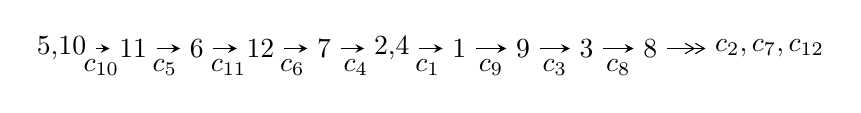
\begin{tikzpicture}[x=23pt, y=7pt]
	% node
	\node (A0) at (-1/8, 0) {5,10};
	\node (A1) at (1, 0) {11};
	\node (A2) at (2, 0) {6};
	\node (A3) at (3, 0) {12};
	\node (A4) at (4, 0) {7};
	\node (A5) at (81/16, 0) {2,4};
	\node (A6) at (49/8, 0) {1};
	\node (A7) at (57/8, 0) {9};
	\node (A8) at (65/8, 0) {3};
	\node (A9) at (73/8, 0) {8};
	\node (C1) at (1/2, -1) {$c_{10}$};
	\node (C2) at (3/2, -1) {$c_{5}$};
	\node (C3) at (5/2, -1) {$c_{11}$};
	\node (C4) at (7/2, -1) {$c_{6}$};
	\node (C5) at (9/2, -1) {$c_{4}$};
	\node (C6) at (45/8, -1) {$c_{1}$};
	\node (C7) at (53/8, -1) {$c_{9}$};
	\node (C8) at (61/8, -1) {$c_{3}$};
	\node (C9) at (69/8, -1) {$c_{8}$};
	\node (A10) at (11, 0) {$c_{2},c_{7},c_{12}$};

	% edge
	\draw[->,>=stealth]	
	(A0) edge (A1) (A1) edge (A2) (A2) edge (A3) (A3) edge (A4) (A4) edge (A5) (A5) edge (A6) (A6) edge (A7) (A7) edge (A8) (A8) edge (A9) ;
	\draw[->>,>={angle 60}]	
	(A9) edge (A10);
\end{tikzpicture} \\ 

\end{tabular} \\

\footnotetext{
The image of knot diagram is generated by the software ``\textbf{Draw programme}" developed by Andrew Bartholomew(\url{http://www.layer8.co.uk/maths/draw/index.htm\#Running-draw}), where we modified some parts for our purpose(\url{https://github.com/CATsTAILs/LinksPainter}).
}\phantom \\ \newline 
\centering \textbf{Ideals for irreducible components\footnotemark of $X_{\text{par}}$} 
 
\begin{align*}
I^u_{1}&=\langle 
3.30422\times10^{51} u^{68}+3.51426\times10^{52} u^{67}+\cdots+1.74141\times10^{53} b-1.35897\times10^{53},\\
\phantom{I^u_{1}}&\phantom{= \langle  }-7.04019\times10^{53} u^{68}+7.16957\times10^{53} u^{67}+\cdots+1.74141\times10^{53} a-5.55666\times10^{54},\;u^{69}- u^{68}+\cdots+16 u+1\rangle \\
I^u_{2}&=\langle 
- u^{12}+9 u^{10}-30 u^8- u^7+45 u^6+5 u^5-29 u^4-7 u^3+6 u^2+b+2 u,\\
\phantom{I^u_{2}}&\phantom{= \langle  }- u^{12}+9 u^{10}-30 u^8-2 u^7+45 u^6+11 u^5-29 u^4-18 u^3+5 u^2+a+8 u+2,\\
\phantom{I^u_{2}}&\phantom{= \langle  }u^{13}-10 u^{11}+38 u^9+u^8-68 u^7-6 u^6+57 u^5+11 u^4-18 u^3-6 u^2+1\rangle \\
\\
\end{align*}
\raggedright * 2 irreducible components of $\dim_{\mathbb{C}}=0$, with total 82 representations.\\
\footnotetext{All coefficients of polynomials are rational numbers. But the coefficients are sometimes approximated in decimal forms when there is not enough margin.}
\newpage
\renewcommand{\arraystretch}{1}
\centering \section*{I. $I^u_{1}= \langle 3.30\times10^{51} u^{68}+3.51\times10^{52} u^{67}+\cdots+1.74\times10^{53} b-1.36\times10^{53},\;-7.04\times10^{53} u^{68}+7.17\times10^{53} u^{67}+\cdots+1.74\times10^{53} a-5.56\times10^{54},\;u^{69}- u^{68}+\cdots+16 u+1 \rangle$}
\flushleft \textbf{(i) Arc colorings}\\
\begin{tabular}{m{7pt} m{180pt} m{7pt} m{180pt} }
\flushright $a_{5}=$&$\begin{pmatrix}0\\u\end{pmatrix}$ \\
\flushright $a_{10}=$&$\begin{pmatrix}1\\0\end{pmatrix}$ \\
\flushright $a_{11}=$&$\begin{pmatrix}1\\u^2\end{pmatrix}$ \\
\flushright $a_{6}=$&$\begin{pmatrix}- u\\- u^3+u\end{pmatrix}$ \\
\flushright $a_{12}=$&$\begin{pmatrix}- u^2+1\\- u^4+2 u^2\end{pmatrix}$ \\
\flushright $a_{7}=$&$\begin{pmatrix}u^3-2 u\\u^5-3 u^3+u\end{pmatrix}$ \\
\flushright $a_{2}=$&$\begin{pmatrix}4.04281 u^{68}-4.11711 u^{67}+\cdots+265.966 u+31.9090\\-0.0189744 u^{68}-0.201805 u^{67}+\cdots+5.33487 u+0.780384\end{pmatrix}$ \\
\flushright $a_{4}=$&$\begin{pmatrix}u\\u\end{pmatrix}$ \\
\flushright $a_{1}=$&$\begin{pmatrix}3.79040 u^{68}-5.00863 u^{67}+\cdots+272.372 u+32.0554\\-0.271387 u^{68}-1.09333 u^{67}+\cdots+11.7404 u+0.926866\end{pmatrix}$ \\
\flushright $a_{9}=$&$\begin{pmatrix}2.63776 u^{68}-3.52798 u^{67}+\cdots+242.870 u+30.7339\\-0.418007 u^{68}-0.165084 u^{67}+\cdots+29.6232 u+2.50226\end{pmatrix}$ \\
\flushright $a_{3}=$&$\begin{pmatrix}3.93419 u^{68}-4.98353 u^{67}+\cdots+286.492 u+33.7569\\-0.370235 u^{68}-0.800602 u^{67}+\cdots+8.34849 u+0.696586\end{pmatrix}$ \\
\flushright $a_{8}=$&$\begin{pmatrix}3.11909 u^{68}-4.03119 u^{67}+\cdots+270.222 u+39.5046\\-0.648080 u^{68}-0.0452525 u^{67}+\cdots+36.0775 u+4.08566\end{pmatrix}$\\&\end{tabular}
\flushleft \textbf{(ii) Obstruction class $= -1$}\\~\\
\flushleft \textbf{(iii) Cusp Shapes $= 6.92150 u^{68}-8.70612 u^{67}+\cdots+422.323 u+41.9072$}\\~\\
\newpage\renewcommand{\arraystretch}{1}
\flushleft \textbf{(iv) u-Polynomials at the component}\newline \\
\begin{tabular}{m{50pt}|m{274pt}}
Crossings & \hspace{64pt}u-Polynomials at each crossing \\
\hline $$\begin{aligned}c_{1}\end{aligned}$$&$\begin{aligned}
&u^{69}-7 u^{68}+\cdots+6887 u-689
\end{aligned}$\\
\hline $$\begin{aligned}c_{2},c_{7}\end{aligned}$$&$\begin{aligned}
&u^{69}-18 u^{67}+\cdots- u-1
\end{aligned}$\\
\hline $$\begin{aligned}c_{3}\end{aligned}$$&$\begin{aligned}
&u^{69}- u^{68}+\cdots+8 u+1
\end{aligned}$\\
\hline $$\begin{aligned}c_{4},c_{5},c_{6}\\c_{10},c_{11}\end{aligned}$$&$\begin{aligned}
&u^{69}+u^{68}+\cdots+16 u-1
\end{aligned}$\\
\hline $$\begin{aligned}c_{8},c_{12}\end{aligned}$$&$\begin{aligned}
&u^{69}-26 u^{67}+\cdots-45 u+29
\end{aligned}$\\
\hline $$\begin{aligned}c_{9}\end{aligned}$$&$\begin{aligned}
&u^{69}+3 u^{68}+\cdots+280 u-139
\end{aligned}$\\
\hline
\end{tabular}\\~\\
\newpage\renewcommand{\arraystretch}{1}
\flushleft \textbf{(v) Riley Polynomials at the component}\newline \\
\begin{tabular}{m{50pt}|m{274pt}}
Crossings & \hspace{64pt}Riley Polynomials at each crossing \\
\hline $$\begin{aligned}c_{1}\end{aligned}$$&$\begin{aligned}
&y^{69}-31 y^{68}+\cdots+26893057 y-474721
\end{aligned}$\\
\hline $$\begin{aligned}c_{2},c_{7}\end{aligned}$$&$\begin{aligned}
&y^{69}-36 y^{68}+\cdots+25 y-1
\end{aligned}$\\
\hline $$\begin{aligned}c_{3}\end{aligned}$$&$\begin{aligned}
&y^{69}+y^{68}+\cdots+16 y-1
\end{aligned}$\\
\hline $$\begin{aligned}c_{4},c_{5},c_{6}\\c_{10},c_{11}\end{aligned}$$&$\begin{aligned}
&y^{69}-95 y^{68}+\cdots+96 y-1
\end{aligned}$\\
\hline $$\begin{aligned}c_{8},c_{12}\end{aligned}$$&$\begin{aligned}
&y^{69}-52 y^{68}+\cdots+25341 y-841
\end{aligned}$\\
\hline $$\begin{aligned}c_{9}\end{aligned}$$&$\begin{aligned}
&y^{69}+17 y^{68}+\cdots-608816 y-19321
\end{aligned}$\\
\hline
\end{tabular}\\~\\
\newpage\flushleft \textbf{(vi) Complex Volumes and Cusp Shapes}
$$\begin{array}{c|c|c}  
\text{Solutions to }I^u_{1}& \I (\text{vol} + \sqrt{-1}CS) & \text{Cusp shape}\\
 \hline 
\begin{aligned}
u &= \phantom{-}0.970523 + 0.108303 I \\
a &= -0.854816 + 1.050670 I \\
b &= -0.104041 + 0.201502 I\end{aligned}
 & -1.13069 - 0.85474 I & \phantom{-0.000000 } 0 \\ \hline\begin{aligned}
u &= \phantom{-}0.970523 - 0.108303 I \\
a &= -0.854816 - 1.050670 I \\
b &= -0.104041 - 0.201502 I\end{aligned}
 & -1.13069 + 0.85474 I & \phantom{-0.000000 } 0 \\ \hline\begin{aligned}
u &= \phantom{-}1.033950 + 0.073948 I \\
a &= -0.51792 - 1.53260 I \\
b &= -1.21908 - 1.48587 I\end{aligned}
 & -5.24202 - 3.64411 I & \phantom{-0.000000 } 0 \\ \hline\begin{aligned}
u &= \phantom{-}1.033950 - 0.073948 I \\
a &= -0.51792 + 1.53260 I \\
b &= -1.21908 + 1.48587 I\end{aligned}
 & -5.24202 + 3.64411 I & \phantom{-0.000000 } 0 \\ \hline\begin{aligned}
u &= -0.960213\phantom{ +0.000000I} \\
a &= \phantom{-}0.604404\phantom{ +0.000000I} \\
b &= -1.23574\phantom{ +0.000000I}\end{aligned}
 & -0.118191\phantom{ +0.000000I} & \phantom{-0.000000 } 0 \\ \hline\begin{aligned}
u &= -0.922631 + 0.233585 I \\
a &= -0.75796 + 1.45099 I \\
b &= \phantom{-}0.403514 + 0.999659 I\end{aligned}
 & -3.71809 + 2.97804 I & \phantom{-0.000000 } 0 \\ \hline\begin{aligned}
u &= -0.922631 - 0.233585 I \\
a &= -0.75796 - 1.45099 I \\
b &= \phantom{-}0.403514 - 0.999659 I\end{aligned}
 & -3.71809 - 2.97804 I & \phantom{-0.000000 } 0 \\ \hline\begin{aligned}
u &= -0.917023 + 0.212783 I \\
a &= \phantom{-}0.08094 + 1.94171 I \\
b &= \phantom{-}0.374010 + 0.305925 I\end{aligned}
 & -2.30574 + 5.04357 I & \phantom{-0.000000 } 0 \\ \hline\begin{aligned}
u &= -0.917023 - 0.212783 I \\
a &= \phantom{-}0.08094 - 1.94171 I \\
b &= \phantom{-}0.374010 - 0.305925 I\end{aligned}
 & -2.30574 - 5.04357 I & \phantom{-0.000000 } 0 \\ \hline\begin{aligned}
u &= -0.900768 + 0.078956 I \\
a &= -0.69952 + 1.99893 I \\
b &= \phantom{-}0.389187 + 1.261770 I\end{aligned}
 & -3.54279 + 2.91613 I & \phantom{-0.000000 } 0\\
 \hline 
 \end{array}$$\newpage$$\begin{array}{c|c|c}  
\text{Solutions to }I^u_{1}& \I (\text{vol} + \sqrt{-1}CS) & \text{Cusp shape}\\
 \hline 
\begin{aligned}
u &= -0.900768 - 0.078956 I \\
a &= -0.69952 - 1.99893 I \\
b &= \phantom{-}0.389187 - 1.261770 I\end{aligned}
 & -3.54279 - 2.91613 I & \phantom{-0.000000 } 0 \\ \hline\begin{aligned}
u &= \phantom{-}1.093250 + 0.272776 I \\
a &= \phantom{-}0.19450 - 1.67030 I \\
b &= \phantom{-}1.09950 - 1.25535 I\end{aligned}
 & -1.31596 - 6.29242 I & \phantom{-0.000000 } 0 \\ \hline\begin{aligned}
u &= \phantom{-}1.093250 - 0.272776 I \\
a &= \phantom{-}0.19450 + 1.67030 I \\
b &= \phantom{-}1.09950 + 1.25535 I\end{aligned}
 & -1.31596 + 6.29242 I & \phantom{-0.000000 } 0 \\ \hline\begin{aligned}
u &= \phantom{-}1.044710 + 0.433897 I \\
a &= \phantom{-}0.686500 + 0.770259 I \\
b &= -0.021208 + 1.131490 I\end{aligned}
 & -5.90299 - 3.46414 I & \phantom{-0.000000 } 0 \\ \hline\begin{aligned}
u &= \phantom{-}1.044710 - 0.433897 I \\
a &= \phantom{-}0.686500 - 0.770259 I \\
b &= -0.021208 - 1.131490 I\end{aligned}
 & -5.90299 + 3.46414 I & \phantom{-0.000000 } 0 \\ \hline\begin{aligned}
u &= \phantom{-}1.127140 + 0.222152 I \\
a &= \phantom{-}0.52291 + 1.41806 I \\
b &= -0.862853 + 0.977792 I\end{aligned}
 & -8.33525 - 5.88314 I & \phantom{-0.000000 } 0 \\ \hline\begin{aligned}
u &= \phantom{-}1.127140 - 0.222152 I \\
a &= \phantom{-}0.52291 - 1.41806 I \\
b &= -0.862853 - 0.977792 I\end{aligned}
 & -8.33525 + 5.88314 I & \phantom{-0.000000 } 0 \\ \hline\begin{aligned}
u &= \phantom{-}0.480235 + 0.689334 I \\
a &= -0.568720 + 0.491028 I \\
b &= -0.450178 - 0.761446 I\end{aligned}
 & -1.51842 + 4.43214 I & \phantom{-0.000000 } 0 \\ \hline\begin{aligned}
u &= \phantom{-}0.480235 - 0.689334 I \\
a &= -0.568720 - 0.491028 I \\
b &= -0.450178 + 0.761446 I\end{aligned}
 & -1.51842 - 4.43214 I & \phantom{-0.000000 } 0 \\ \hline\begin{aligned}
u &= -1.115900 + 0.395594 I \\
a &= \phantom{-}0.24502 - 1.47620 I \\
b &= -1.00488 - 1.21839 I\end{aligned}
 & -5.66016 + 12.60390 I & \phantom{-0.000000 } 0\\
 \hline 
 \end{array}$$\newpage$$\begin{array}{c|c|c}  
\text{Solutions to }I^u_{1}& \I (\text{vol} + \sqrt{-1}CS) & \text{Cusp shape}\\
 \hline 
\begin{aligned}
u &= -1.115900 - 0.395594 I \\
a &= \phantom{-}0.24502 + 1.47620 I \\
b &= -1.00488 + 1.21839 I\end{aligned}
 & -5.66016 - 12.60390 I & \phantom{-0.000000 } 0 \\ \hline\begin{aligned}
u &= \phantom{-}0.337583 + 0.691942 I \\
a &= -0.659876 - 0.083894 I \\
b &= \phantom{-}0.778722 - 0.958452 I\end{aligned}
 & -1.13098 - 8.91114 I & -4.00000 + 8.49340 I \\ \hline\begin{aligned}
u &= \phantom{-}0.337583 - 0.691942 I \\
a &= -0.659876 + 0.083894 I \\
b &= \phantom{-}0.778722 + 0.958452 I\end{aligned}
 & -1.13098 + 8.91114 I & -4.00000 - 8.49340 I \\ \hline\begin{aligned}
u &= -1.278510 + 0.014060 I \\
a &= -0.530795 - 0.268501 I \\
b &= -1.083720 - 0.300872 I\end{aligned}
 & -7.37922 - 0.04313 I & \phantom{-0.000000 } 0 \\ \hline\begin{aligned}
u &= -1.278510 - 0.014060 I \\
a &= -0.530795 + 0.268501 I \\
b &= -1.083720 + 0.300872 I\end{aligned}
 & -7.37922 + 0.04313 I & \phantom{-0.000000 } 0 \\ \hline\begin{aligned}
u &= \phantom{-}0.655716 + 0.240239 I \\
a &= -0.291654 - 0.184454 I \\
b &= \phantom{-}0.966260 + 0.067900 I\end{aligned}
 & -1.031510 + 0.312804 I & -8.34035 + 1.35782 I \\ \hline\begin{aligned}
u &= \phantom{-}0.655716 - 0.240239 I \\
a &= -0.291654 + 0.184454 I \\
b &= \phantom{-}0.966260 - 0.067900 I\end{aligned}
 & -1.031510 - 0.312804 I & -8.34035 - 1.35782 I \\ \hline\begin{aligned}
u &= -0.165954 + 0.649062 I \\
a &= \phantom{-}0.003498 - 0.456639 I \\
b &= -0.255335 + 0.985701 I\end{aligned}
 & -2.17679 - 0.26649 I & -8.08515 - 0.77789 I \\ \hline\begin{aligned}
u &= -0.165954 - 0.649062 I \\
a &= \phantom{-}0.003498 + 0.456639 I \\
b &= -0.255335 - 0.985701 I\end{aligned}
 & -2.17679 + 0.26649 I & -8.08515 + 0.77789 I \\ \hline\begin{aligned}
u &= -0.468363 + 0.413877 I \\
a &= -1.59539 + 0.60353 I \\
b &= \phantom{-}0.496715 + 0.910892 I\end{aligned}
 & -3.36016 + 3.70048 I & -9.81035 - 6.09222 I\\
 \hline 
 \end{array}$$\newpage$$\begin{array}{c|c|c}  
\text{Solutions to }I^u_{1}& \I (\text{vol} + \sqrt{-1}CS) & \text{Cusp shape}\\
 \hline 
\begin{aligned}
u &= -0.468363 - 0.413877 I \\
a &= -1.59539 - 0.60353 I \\
b &= \phantom{-}0.496715 - 0.910892 I\end{aligned}
 & -3.36016 - 3.70048 I & -9.81035 + 6.09222 I \\ \hline\begin{aligned}
u &= -1.337030 + 0.327168 I \\
a &= \phantom{-}0.464853 - 0.302329 I \\
b &= -0.078909 - 0.591498 I\end{aligned}
 & -7.29700 - 0.75484 I & \phantom{-0.000000 } 0 \\ \hline\begin{aligned}
u &= -1.337030 - 0.327168 I \\
a &= \phantom{-}0.464853 + 0.302329 I \\
b &= -0.078909 + 0.591498 I\end{aligned}
 & -7.29700 + 0.75484 I & \phantom{-0.000000 } 0 \\ \hline\begin{aligned}
u &= \phantom{-}0.607599\phantom{ +0.000000I} \\
a &= -0.226329\phantom{ +0.000000I} \\
b &= \phantom{-}0.516562\phantom{ +0.000000I}\end{aligned}
 & -1.12956\phantom{ +0.000000I} & -8.41060\phantom{ +0.000000I} \\ \hline\begin{aligned}
u &= -0.314959 + 0.499815 I \\
a &= \phantom{-}0.599510 - 0.307709 I \\
b &= -0.951155 - 0.796839 I\end{aligned}
 & \phantom{-}3.10870 + 3.65525 I & -0.44555 - 7.33044 I \\ \hline\begin{aligned}
u &= -0.314959 - 0.499815 I \\
a &= \phantom{-}0.599510 + 0.307709 I \\
b &= -0.951155 + 0.796839 I\end{aligned}
 & \phantom{-}3.10870 - 3.65525 I & -0.44555 + 7.33044 I \\ \hline\begin{aligned}
u &= -0.371311 + 0.394330 I \\
a &= \phantom{-}0.97740 + 1.13892 I \\
b &= \phantom{-}0.739429 - 0.343891 I\end{aligned}
 & \phantom{-}2.88878 - 0.59529 I & \phantom{-}0.335042 - 1.258913 I \\ \hline\begin{aligned}
u &= -0.371311 - 0.394330 I \\
a &= \phantom{-}0.97740 - 1.13892 I \\
b &= \phantom{-}0.739429 + 0.343891 I\end{aligned}
 & \phantom{-}2.88878 + 0.59529 I & \phantom{-}0.335042 + 1.258913 I \\ \hline\begin{aligned}
u &= \phantom{-}1.51600\phantom{ +0.000000I} \\
a &= -0.972604\phantom{ +0.000000I} \\
b &= -0.823418\phantom{ +0.000000I}\end{aligned}
 & -3.18079\phantom{ +0.000000I} & \phantom{-0.000000 } 0 \\ \hline\begin{aligned}
u &= \phantom{-}0.083281 + 0.453009 I \\
a &= \phantom{-}1.35995 + 1.51466 I \\
b &= -0.724939 + 0.127054 I\end{aligned}
 & \phantom{-}0.70817 - 2.77944 I & -0.09198 + 6.13173 I\\
 \hline 
 \end{array}$$\newpage$$\begin{array}{c|c|c}  
\text{Solutions to }I^u_{1}& \I (\text{vol} + \sqrt{-1}CS) & \text{Cusp shape}\\
 \hline 
\begin{aligned}
u &= \phantom{-}0.083281 - 0.453009 I \\
a &= \phantom{-}1.35995 - 1.51466 I \\
b &= -0.724939 - 0.127054 I\end{aligned}
 & \phantom{-}0.70817 + 2.77944 I & -0.09198 - 6.13173 I \\ \hline\begin{aligned}
u &= \phantom{-}0.195749 + 0.351698 I \\
a &= \phantom{-}1.169440 - 0.099926 I \\
b &= -0.278714 + 0.641393 I\end{aligned}
 & -0.314860 - 1.014580 I & -5.61645 + 6.17705 I \\ \hline\begin{aligned}
u &= \phantom{-}0.195749 - 0.351698 I \\
a &= \phantom{-}1.169440 + 0.099926 I \\
b &= -0.278714 - 0.641393 I\end{aligned}
 & -0.314860 + 1.014580 I & -5.61645 - 6.17705 I \\ \hline\begin{aligned}
u &= -1.66089\phantom{ +0.000000I} \\
a &= -0.179607\phantom{ +0.000000I} \\
b &= -1.14488\phantom{ +0.000000I}\end{aligned}
 & -9.16005\phantom{ +0.000000I} & \phantom{-0.000000 } 0 \\ \hline\begin{aligned}
u &= \phantom{-}1.70441 + 0.07129 I \\
a &= \phantom{-}0.22559 + 1.66331 I \\
b &= -0.494925 + 1.140110 I\end{aligned}
 & -13.04310 - 4.25845 I & \phantom{-0.000000 } 0 \\ \hline\begin{aligned}
u &= \phantom{-}1.70441 - 0.07129 I \\
a &= \phantom{-}0.22559 - 1.66331 I \\
b &= -0.494925 - 1.140110 I\end{aligned}
 & -13.04310 + 4.25845 I & \phantom{-0.000000 } 0 \\ \hline\begin{aligned}
u &= \phantom{-}1.70688 + 0.04723 I \\
a &= -0.15217 + 1.71603 I \\
b &= -0.216141 + 0.574577 I\end{aligned}
 & -11.67470 - 6.01387 I & \phantom{-0.000000 } 0 \\ \hline\begin{aligned}
u &= \phantom{-}1.70688 - 0.04723 I \\
a &= -0.15217 - 1.71603 I \\
b &= -0.216141 - 0.574577 I\end{aligned}
 & -11.67470 + 6.01387 I & \phantom{-0.000000 } 0 \\ \hline\begin{aligned}
u &= \phantom{-}1.71727 + 0.01724 I \\
a &= -0.14976 + 2.06323 I \\
b &= -0.76930 + 1.55036 I\end{aligned}
 & -13.04020 - 3.28190 I & \phantom{-0.000000 } 0 \\ \hline\begin{aligned}
u &= \phantom{-}1.71727 - 0.01724 I \\
a &= -0.14976 - 2.06323 I \\
b &= -0.76930 - 1.55036 I\end{aligned}
 & -13.04020 + 3.28190 I & \phantom{-0.000000 } 0\\
 \hline 
 \end{array}$$\newpage$$\begin{array}{c|c|c}  
\text{Solutions to }I^u_{1}& \I (\text{vol} + \sqrt{-1}CS) & \text{Cusp shape}\\
 \hline 
\begin{aligned}
u &= -1.72043 + 0.01720 I \\
a &= \phantom{-}0.319134 + 1.230620 I \\
b &= -0.152732 + 0.585019 I\end{aligned}
 & -10.78490 + 1.28215 I & \phantom{-0.000000 } 0 \\ \hline\begin{aligned}
u &= -1.72043 - 0.01720 I \\
a &= \phantom{-}0.319134 - 1.230620 I \\
b &= -0.152732 - 0.585019 I\end{aligned}
 & -10.78490 - 1.28215 I & \phantom{-0.000000 } 0 \\ \hline\begin{aligned}
u &= \phantom{-}1.72209\phantom{ +0.000000I} \\
a &= \phantom{-}0.327354\phantom{ +0.000000I} \\
b &= \phantom{-}1.49160\phantom{ +0.000000I}\end{aligned}
 & -9.78852\phantom{ +0.000000I} & \phantom{-0.000000 } 0 \\ \hline\begin{aligned}
u &= -1.73799 + 0.01931 I \\
a &= \phantom{-}1.08020 - 1.84615 I \\
b &= \phantom{-}1.55088 - 1.72505 I\end{aligned}
 & -15.2509 + 4.0310 I & \phantom{-0.000000 } 0 \\ \hline\begin{aligned}
u &= -1.73799 - 0.01931 I \\
a &= \phantom{-}1.08020 + 1.84615 I \\
b &= \phantom{-}1.55088 + 1.72505 I\end{aligned}
 & -15.2509 - 4.0310 I & \phantom{-0.000000 } 0 \\ \hline\begin{aligned}
u &= -1.74421 + 0.11729 I \\
a &= -0.28874 + 1.41097 I \\
b &= \phantom{-}0.263478 + 1.336250 I\end{aligned}
 & -15.7999 + 5.7580 I & \phantom{-0.000000 } 0 \\ \hline\begin{aligned}
u &= -1.74421 - 0.11729 I \\
a &= -0.28874 - 1.41097 I \\
b &= \phantom{-}0.263478 - 1.336250 I\end{aligned}
 & -15.7999 - 5.7580 I & \phantom{-0.000000 } 0 \\ \hline\begin{aligned}
u &= -1.75104 + 0.07156 I \\
a &= -0.67507 - 1.98321 I \\
b &= -1.25654 - 1.57527 I\end{aligned}
 & -11.53150 + 7.74332 I & \phantom{-0.000000 } 0 \\ \hline\begin{aligned}
u &= -1.75104 - 0.07156 I \\
a &= -0.67507 + 1.98321 I \\
b &= -1.25654 + 1.57527 I\end{aligned}
 & -11.53150 - 7.74332 I & \phantom{-0.000000 } 0 \\ \hline\begin{aligned}
u &= -1.75568 + 0.05812 I \\
a &= \phantom{-}0.13855 + 1.50571 I \\
b &= \phantom{-}1.11222 + 1.06448 I\end{aligned}
 & -18.7148 + 7.0816 I & \phantom{-0.000000 } 0\\
 \hline 
 \end{array}$$\newpage$$\begin{array}{c|c|c}  
\text{Solutions to }I^u_{1}& \I (\text{vol} + \sqrt{-1}CS) & \text{Cusp shape}\\
 \hline 
\begin{aligned}
u &= -1.75568 - 0.05812 I \\
a &= \phantom{-}0.13855 - 1.50571 I \\
b &= \phantom{-}1.11222 - 1.06448 I\end{aligned}
 & -18.7148 - 7.0816 I & \phantom{-0.000000 } 0 \\ \hline\begin{aligned}
u &= \phantom{-}1.75461 + 0.10664 I \\
a &= \phantom{-}0.32391 - 1.84018 I \\
b &= \phantom{-}1.17322 - 1.41872 I\end{aligned}
 & -15.8746 - 14.7349 I & \phantom{-0.000000 } 0 \\ \hline\begin{aligned}
u &= \phantom{-}1.75461 - 0.10664 I \\
a &= \phantom{-}0.32391 + 1.84018 I \\
b &= \phantom{-}1.17322 + 1.41872 I\end{aligned}
 & -15.8746 + 14.7349 I & \phantom{-0.000000 } 0 \\ \hline\begin{aligned}
u &= \phantom{-}1.79142 + 0.04126 I \\
a &= \phantom{-}0.376682 - 0.961683 I \\
b &= \phantom{-}0.885083 - 0.907630 I\end{aligned}
 & -18.8425 - 0.5002 I & \phantom{-0.000000 } 0 \\ \hline\begin{aligned}
u &= \phantom{-}1.79142 - 0.04126 I \\
a &= \phantom{-}0.376682 + 0.961683 I \\
b &= \phantom{-}0.885083 + 0.907630 I\end{aligned}
 & -18.8425 + 0.5002 I & \phantom{-0.000000 } 0 \\ \hline\begin{aligned}
u &= -0.153507 + 0.114938 I \\
a &= -3.62976 - 1.49255 I \\
b &= \phantom{-}0.550095 - 1.156120 I\end{aligned}
 & -1.43627 + 2.95426 I & -9.8137 - 11.3357 I \\ \hline\begin{aligned}
u &= -0.153507 - 0.114938 I \\
a &= -3.62976 + 1.49255 I \\
b &= \phantom{-}0.550095 + 1.156120 I\end{aligned}
 & -1.43627 - 2.95426 I & -9.8137 + 11.3357 I \\ \hline\begin{aligned}
u &= \phantom{-}1.80975\phantom{ +0.000000I} \\
a &= \phantom{-}1.20100\phantom{ +0.000000I} \\
b &= \phantom{-}1.65732\phantom{ +0.000000I}\end{aligned}
 & -18.8871\phantom{ +0.000000I} & \phantom{-0.000000 } 0 \\ \hline\begin{aligned}
u &= -0.117170\phantom{ +0.000000I} \\
a &= \phantom{-}11.4529\phantom{ +0.000000I} \\
b &= \phantom{-}0.823225\phantom{ +0.000000I}\end{aligned}
 & \phantom{-}2.72284\phantom{ +0.000000I} & \phantom{-}13.1210\phantom{ +0.000000I}\\
 \hline 
 \end{array}$$\newpage\newpage\renewcommand{\arraystretch}{1}
\centering \section*{II. $I^u_{2}= \langle - u^{12}+9 u^{10}+\cdots+b+2 u,\;- u^{12}+9 u^{10}+\cdots+a+2,\;u^{13}-10 u^{11}+\cdots-6 u^2+1 \rangle$}
\flushleft \textbf{(i) Arc colorings}\\
\begin{tabular}{m{7pt} m{180pt} m{7pt} m{180pt} }
\flushright $a_{5}=$&$\begin{pmatrix}0\\u\end{pmatrix}$ \\
\flushright $a_{10}=$&$\begin{pmatrix}1\\0\end{pmatrix}$ \\
\flushright $a_{11}=$&$\begin{pmatrix}1\\u^2\end{pmatrix}$ \\
\flushright $a_{6}=$&$\begin{pmatrix}- u\\- u^3+u\end{pmatrix}$ \\
\flushright $a_{12}=$&$\begin{pmatrix}- u^2+1\\- u^4+2 u^2\end{pmatrix}$ \\
\flushright $a_{7}=$&$\begin{pmatrix}u^3-2 u\\u^5-3 u^3+u\end{pmatrix}$ \\
\flushright $a_{2}=$&$\begin{pmatrix}u^{12}-9 u^{10}+30 u^8+2 u^7-45 u^6-11 u^5+29 u^4+18 u^3-5 u^2-8 u-2\\u^{12}-9 u^{10}+30 u^8+u^7-45 u^6-5 u^5+29 u^4+7 u^3-6 u^2-2 u\end{pmatrix}$ \\
\flushright $a_{4}=$&$\begin{pmatrix}u\\u\end{pmatrix}$ \\
\flushright $a_{1}=$&$\begin{pmatrix}u^{12}-9 u^{10}+\cdots-8 u-2\\u^{12}-9 u^{10}- u^9+30 u^8+7 u^7-45 u^6-16 u^5+28 u^4+13 u^3-4 u^2-2 u\end{pmatrix}$ \\
\flushright $a_{9}=$&$\begin{pmatrix}- u^{12}+10 u^{10}-37 u^8- u^7+61 u^6+6 u^5-41 u^4-11 u^3+5 u^2+5 u+3\\- u^3+2 u\end{pmatrix}$ \\
\flushright $a_{3}=$&$\begin{pmatrix}u^{12}-9 u^{10}+\cdots-10 u-3\\u^{12}-9 u^{10}+30 u^8+u^7-45 u^6-5 u^5+29 u^4+7 u^3-6 u^2- u\end{pmatrix}$ \\
\flushright $a_{8}=$&$\begin{pmatrix}- u^{12}+10 u^{10}+\cdots+11 u+4\\u^{11}-8 u^9- u^8+23 u^7+7 u^6-28 u^5-15 u^4+11 u^3+10 u^2+2 u-1\end{pmatrix}$\\&\end{tabular}
\flushleft \textbf{(ii) Obstruction class $= 1$}\\~\\
\flushleft \textbf{(iii) Cusp Shapes $= u^{12}+5 u^{11}-10 u^{10}-44 u^9+41 u^8+143 u^7-80 u^6-210 u^5+62 u^4+133 u^3-23 u-17$}\\~\\
\newpage\renewcommand{\arraystretch}{1}
\flushleft \textbf{(iv) u-Polynomials at the component}\newline \\
\begin{tabular}{m{50pt}|m{274pt}}
Crossings & \hspace{64pt}u-Polynomials at each crossing \\
\hline $$\begin{aligned}c_{1}\end{aligned}$$&$\begin{aligned}
&u^{13}-4 u^{11}+\cdots+5 u-1
\end{aligned}$\\
\hline $$\begin{aligned}c_{2}\end{aligned}$$&$\begin{aligned}
&u^{13}+u^{12}+\cdots+u+1
\end{aligned}$\\
\hline $$\begin{aligned}c_{3}\end{aligned}$$&$\begin{aligned}
&u^{13}-2 u^{11}- u^{10}-2 u^9-3 u^8+u^6+u^5+4 u^4+u^3-1
\end{aligned}$\\
\hline $$\begin{aligned}c_{4},c_{5},c_{6}\end{aligned}$$&$\begin{aligned}
&u^{13}-10 u^{11}+38 u^9- u^8-68 u^7+6 u^6+57 u^5-11 u^4-18 u^3+6 u^2-1
\end{aligned}$\\
\hline $$\begin{aligned}c_{7}\end{aligned}$$&$\begin{aligned}
&u^{13}- u^{12}+\cdots+u-1
\end{aligned}$\\
\hline $$\begin{aligned}c_{8}\end{aligned}$$&$\begin{aligned}
&u^{13}- u^{12}+\cdots+u-1
\end{aligned}$\\
\hline $$\begin{aligned}c_{9}\end{aligned}$$&$\begin{aligned}
&u^{13}- u^{10}-4 u^9- u^8- u^7+3 u^5+2 u^4+u^3+2 u^2-1
\end{aligned}$\\
\hline $$\begin{aligned}c_{10},c_{11}\end{aligned}$$&$\begin{aligned}
&u^{13}-10 u^{11}+38 u^9+u^8-68 u^7-6 u^6+57 u^5+11 u^4-18 u^3-6 u^2+1
\end{aligned}$\\
\hline $$\begin{aligned}c_{12}\end{aligned}$$&$\begin{aligned}
&u^{13}+u^{12}+\cdots+u+1
\end{aligned}$\\
\hline
\end{tabular}\\~\\
\newpage\renewcommand{\arraystretch}{1}
\flushleft \textbf{(v) Riley Polynomials at the component}\newline \\
\begin{tabular}{m{50pt}|m{274pt}}
Crossings & \hspace{64pt}Riley Polynomials at each crossing \\
\hline $$\begin{aligned}c_{1}\end{aligned}$$&$\begin{aligned}
&y^{13}-8 y^{12}+\cdots+9 y-1
\end{aligned}$\\
\hline $$\begin{aligned}c_{2},c_{7}\end{aligned}$$&$\begin{aligned}
&y^{13}-13 y^{12}+\cdots+13 y-1
\end{aligned}$\\
\hline $$\begin{aligned}c_{3}\end{aligned}$$&$\begin{aligned}
&y^{13}-4 y^{12}+7 y^{10}-9 y^8+6 y^7+19 y^6-9 y^5-20 y^4+3 y^3+8 y^2-1
\end{aligned}$\\
\hline $$\begin{aligned}c_{4},c_{5},c_{6}\\c_{10},c_{11}\end{aligned}$$&$\begin{aligned}
&y^{13}-20 y^{12}+\cdots+12 y-1
\end{aligned}$\\
\hline $$\begin{aligned}c_{8},c_{12}\end{aligned}$$&$\begin{aligned}
&y^{13}-13 y^{12}+\cdots+13 y-1
\end{aligned}$\\
\hline $$\begin{aligned}c_{9}\end{aligned}$$&$\begin{aligned}
&y^{13}-8 y^{11}-3 y^{10}+20 y^9+9 y^8-19 y^7-6 y^6+9 y^5-7 y^3+4 y-1
\end{aligned}$\\
\hline
\end{tabular}\\~\\
\newpage\flushleft \textbf{(vi) Complex Volumes and Cusp Shapes}
$$\begin{array}{c|c|c}  
\text{Solutions to }I^u_{2}& \I (\text{vol} + \sqrt{-1}CS) & \text{Cusp shape}\\
 \hline 
\begin{aligned}
u &= -0.900642 + 0.211290 I \\
a &= -0.89953 + 1.86106 I \\
b &= -0.037612 + 1.092140 I\end{aligned}
 & -3.44781 + 4.22361 I & -9.99869 - 7.63221 I \\ \hline\begin{aligned}
u &= -0.900642 - 0.211290 I \\
a &= -0.89953 - 1.86106 I \\
b &= -0.037612 - 1.092140 I\end{aligned}
 & -3.44781 - 4.22361 I & -9.99869 + 7.63221 I \\ \hline\begin{aligned}
u &= \phantom{-}0.835287\phantom{ +0.000000I} \\
a &= -1.01640\phantom{ +0.000000I} \\
b &= \phantom{-}1.04297\phantom{ +0.000000I}\end{aligned}
 & \phantom{-}0.774317\phantom{ +0.000000I} & -0.352240\phantom{ +0.000000I} \\ \hline\begin{aligned}
u &= \phantom{-}1.349780 + 0.188354 I \\
a &= -0.360972 + 0.236906 I \\
b &= -0.753544 + 0.428711 I\end{aligned}
 & -6.62178 + 0.41146 I & -4.17258 - 0.90590 I \\ \hline\begin{aligned}
u &= \phantom{-}1.349780 - 0.188354 I \\
a &= -0.360972 - 0.236906 I \\
b &= -0.753544 - 0.428711 I\end{aligned}
 & -6.62178 - 0.41146 I & -4.17258 + 0.90590 I \\ \hline\begin{aligned}
u &= -1.48165\phantom{ +0.000000I} \\
a &= \phantom{-}1.01148\phantom{ +0.000000I} \\
b &= \phantom{-}0.537900\phantom{ +0.000000I}\end{aligned}
 & -3.72558\phantom{ +0.000000I} & -14.4700\phantom{ +0.000000I} \\ \hline\begin{aligned}
u &= -0.246497 + 0.330591 I \\
a &= \phantom{-}0.528174 - 0.970691 I \\
b &= \phantom{-}0.379862 + 0.838529 I\end{aligned}
 & -1.26239 - 2.39614 I & -4.80417 - 1.14749 I \\ \hline\begin{aligned}
u &= -0.246497 - 0.330591 I \\
a &= \phantom{-}0.528174 + 0.970691 I \\
b &= \phantom{-}0.379862 - 0.838529 I\end{aligned}
 & -1.26239 + 2.39614 I & -4.80417 + 1.14749 I \\ \hline\begin{aligned}
u &= \phantom{-}0.333287\phantom{ +0.000000I} \\
a &= -4.29907\phantom{ +0.000000I} \\
b &= -0.793443\phantom{ +0.000000I}\end{aligned}
 & \phantom{-}2.47324\phantom{ +0.000000I} & -19.8810\phantom{ +0.000000I} \\ \hline\begin{aligned}
u &= -1.68760\phantom{ +0.000000I} \\
a &= \phantom{-}0.0537118\phantom{ +0.000000I} \\
b &= -1.19628\phantom{ +0.000000I}\end{aligned}
 & -8.25610\phantom{ +0.000000I} & -1.28480\phantom{ +0.000000I}\\
 \hline 
 \end{array}$$\newpage$$\begin{array}{c|c|c}  
\text{Solutions to }I^u_{2}& \I (\text{vol} + \sqrt{-1}CS) & \text{Cusp shape}\\
 \hline 
\begin{aligned}
u &= \phantom{-}1.70777 + 0.05845 I \\
a &= \phantom{-}0.29300 + 1.93652 I \\
b &= -0.157231 + 1.253940 I\end{aligned}
 & -12.79170 - 5.30924 I & -11.13586 + 5.88346 I \\ \hline\begin{aligned}
u &= \phantom{-}1.70777 - 0.05845 I \\
a &= \phantom{-}0.29300 - 1.93652 I \\
b &= -0.157231 - 1.253940 I\end{aligned}
 & -12.79170 + 5.30924 I & -11.13586 - 5.88346 I \\ \hline\begin{aligned}
u &= -1.82016\phantom{ +0.000000I} \\
a &= \phantom{-}1.12892\phantom{ +0.000000I} \\
b &= \phantom{-}1.54590\phantom{ +0.000000I}\end{aligned}
 & -18.6855\phantom{ +0.000000I} & \phantom{-}11.2100\phantom{ +0.000000I}\\
 \hline 
 \end{array}$$\newpage
\newpage\renewcommand{\arraystretch}{1}
\centering \section*{ III. u-Polynomials}
\begin{tabular}{m{50pt}|m{274pt}}
Crossings & \hspace{64pt}u-Polynomials at each crossing \\
\hline $$\begin{aligned}c_{1}\end{aligned}$$&$\begin{aligned}
&(u^{13}-4 u^{11}+\cdots+5 u-1)(u^{69}-7 u^{68}+\cdots+6887 u-689)
\end{aligned}$\\
\hline $$\begin{aligned}c_{2}\end{aligned}$$&$\begin{aligned}
&(u^{13}+u^{12}+\cdots+u+1)(u^{69}-18 u^{67}+\cdots- u-1)
\end{aligned}$\\
\hline $$\begin{aligned}c_{3}\end{aligned}$$&$\begin{aligned}
&(u^{13}-2 u^{11}- u^{10}-2 u^9-3 u^8+u^6+u^5+4 u^4+u^3-1)\\
&\cdot(u^{69}- u^{68}+\cdots+8 u+1)
\end{aligned}$\\
\hline $$\begin{aligned}c_{4},c_{5},c_{6}\end{aligned}$$&$\begin{aligned}
&(u^{13}-10 u^{11}+38 u^9- u^8-68 u^7+6 u^6+57 u^5-11 u^4-18 u^3+6 u^2-1)\\
&\cdot(u^{69}+u^{68}+\cdots+16 u-1)
\end{aligned}$\\
\hline $$\begin{aligned}c_{7}\end{aligned}$$&$\begin{aligned}
&(u^{13}- u^{12}+\cdots+u-1)(u^{69}-18 u^{67}+\cdots- u-1)
\end{aligned}$\\
\hline $$\begin{aligned}c_{8}\end{aligned}$$&$\begin{aligned}
&(u^{13}- u^{12}+\cdots+u-1)(u^{69}-26 u^{67}+\cdots-45 u+29)
\end{aligned}$\\
\hline $$\begin{aligned}c_{9}\end{aligned}$$&$\begin{aligned}
&(u^{13}- u^{10}-4 u^9- u^8- u^7+3 u^5+2 u^4+u^3+2 u^2-1)\\
&\cdot(u^{69}+3 u^{68}+\cdots+280 u-139)
\end{aligned}$\\
\hline $$\begin{aligned}c_{10},c_{11}\end{aligned}$$&$\begin{aligned}
&(u^{13}-10 u^{11}+38 u^9+u^8-68 u^7-6 u^6+57 u^5+11 u^4-18 u^3-6 u^2+1)\\
&\cdot(u^{69}+u^{68}+\cdots+16 u-1)
\end{aligned}$\\
\hline $$\begin{aligned}c_{12}\end{aligned}$$&$\begin{aligned}
&(u^{13}+u^{12}+\cdots+u+1)(u^{69}-26 u^{67}+\cdots-45 u+29)
\end{aligned}$\\
\hline
\end{tabular}\newpage\renewcommand{\arraystretch}{1}
\centering \section*{ IV. Riley Polynomials}
\begin{tabular}{m{50pt}|m{274pt}}
Crossings & \hspace{64pt}Riley Polynomials at each crossing \\
\hline $$\begin{aligned}c_{1}\end{aligned}$$&$\begin{aligned}
&(y^{13}-8 y^{12}+\cdots+9 y-1)(y^{69}-31 y^{68}+\cdots+2.68931\times10^{7} y-474721)
\end{aligned}$\\
\hline $$\begin{aligned}c_{2},c_{7}\end{aligned}$$&$\begin{aligned}
&(y^{13}-13 y^{12}+\cdots+13 y-1)(y^{69}-36 y^{68}+\cdots+25 y-1)
\end{aligned}$\\
\hline $$\begin{aligned}c_{3}\end{aligned}$$&$\begin{aligned}
&(y^{13}-4 y^{12}+7 y^{10}-9 y^8+6 y^7+19 y^6-9 y^5-20 y^4+3 y^3+8 y^2-1)\\
&\cdot(y^{69}+y^{68}+\cdots+16 y-1)
\end{aligned}$\\
\hline $$\begin{aligned}c_{4},c_{5},c_{6}\\c_{10},c_{11}\end{aligned}$$&$\begin{aligned}
&(y^{13}-20 y^{12}+\cdots+12 y-1)(y^{69}-95 y^{68}+\cdots+96 y-1)
\end{aligned}$\\
\hline $$\begin{aligned}c_{8},c_{12}\end{aligned}$$&$\begin{aligned}
&(y^{13}-13 y^{12}+\cdots+13 y-1)(y^{69}-52 y^{68}+\cdots+25341 y-841)
\end{aligned}$\\
\hline $$\begin{aligned}c_{9}\end{aligned}$$&$\begin{aligned}
&(y^{13}-8 y^{11}-3 y^{10}+20 y^9+9 y^8-19 y^7-6 y^6+9 y^5-7 y^3+4 y-1)\\
&\cdot(y^{69}+17 y^{68}+\cdots-608816 y-19321)
\end{aligned}$\\
\hline
\end{tabular}
\vskip 2pc
\end{document}